\documentclass[twocolumn, 11pt]{article}%
\usepackage{amsmath, amssymb, esint, gensymb, hyperref, mathtools}
\usepackage{graphicx, cuted, geometry, float, scalerel, xcolor, xfrac}
\usepackage{enumitem}


\geometry{
    a4paper,
    total={170mm,260mm},
}

\begin{document}

\begin{strip}
  \vspace*{\dimexpr-\stripsep}
  \begin{center}
      \Large\textbf{FISIKA 2}\\
      \large{Pertemuan 1 - Minggu 11 (423608)}\\
      \large{\today}
   \end{center}
\end{strip}

\section{Arus Bolak Balik}

\subsection{Arus DC}%
Dalam arus DC, nilai dan arah arus selalu tetap (tinjauan nilai tetap
selama tidak ada pengaruh transient).

Gejala transien adalah gejala yang terjadi dalam selang waktu yang pendek
pada saat rangkaian yang berisi resistor (R) dan atau kapasitor (C) dan
Induktor (L) diputus dan disambungkan dengan sumber tegangan.

\subsection{Arus AC}%
Dalam arus AC, nilai dan arah arus berubah terhadap waktu secara
periodik.

\begin{center}
    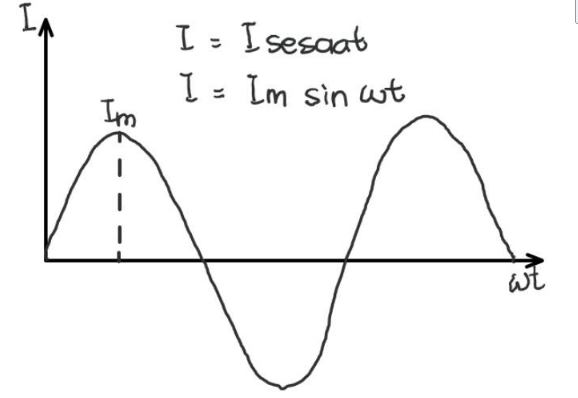
\includegraphics[width=200px]{1.png}
\end{center}

Dengan menggunakan pengukuran osiloskop, dapat diperoleh hubungan arus
terhadap waktu.

\[ V_{\text{RMS}} = \frac{V_{max}}{\sqrt2} \]

\begin{center}
    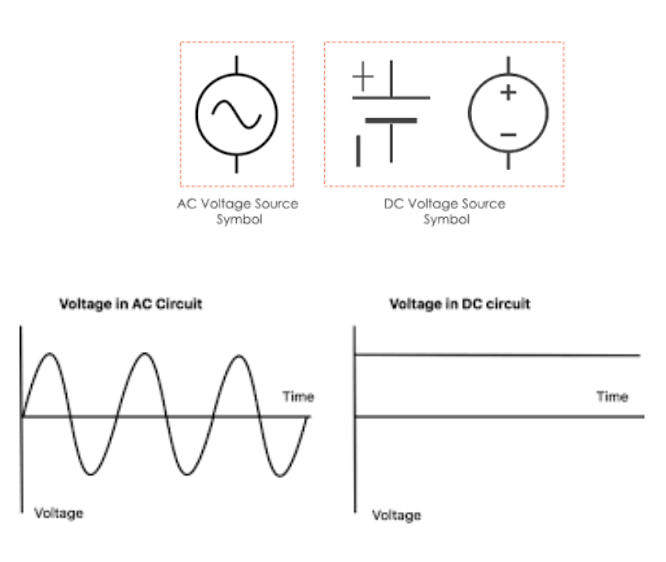
\includegraphics[width=200px]{2.png}
\end{center}

\section{Resistansi dalam rangkaian AC}%

\begin{center}
    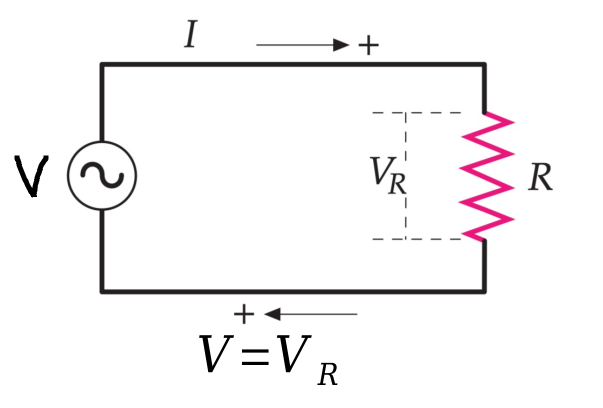
\includegraphics[width=180px]{3.png}
\end{center}

Dalam rangkaian di atas,
\[ V=V_m \sin (\omega t) \]

Dengan, $V-IR=0$

Untuk arus yang mengalir pada rangkaian di atas adalah
\begin{align*}
    IR &= V_m (\sin \omega t)\\
    I &= \frac{V_m}{R}(\sin \omega t)\\
    I &=I_m \sin (\omega t)
\end{align*}

\begin{center}
    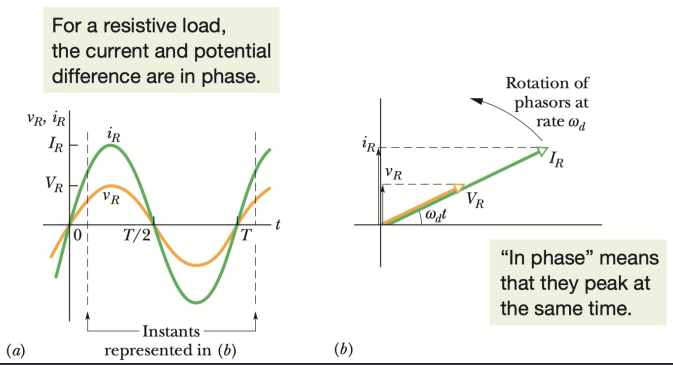
\includegraphics[width=200px]{4.png}
\end{center}

\section{Induktansi Dalam Rangkaian Bolak-balik}%

\begin{center}
    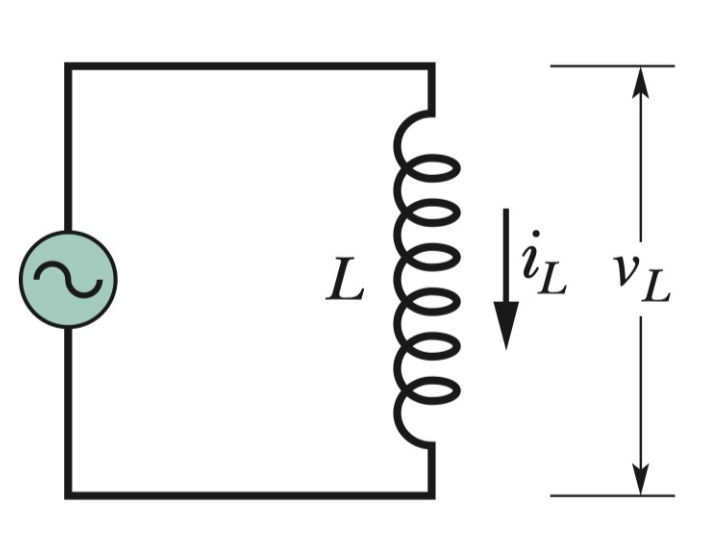
\includegraphics[width=160px]{5.png}
\end{center}

Dalam rangkaian di atas,
\[ V=V_m \sin (\omega t)\]

Dengan, $\displaystyle V-L\frac{dI}{dt}=0$

Maka,

\begin{align*}
    L\frac{dI}{dt}&=V\\
    L\frac{dI}{dt}&=V_{\text{max}}\sin(\omega t)\\
    dI&=\frac{V_{\text{max}}}{L}\sin(\omega t)\ dt\\
    I&=\frac{V_{\text{max}}}{L}\int_0^t\sin(\omega t)\ dt\\
    I&=\frac{V_{\text{max}}}{\omega L}-\cos(\omega t)\\
\end{align*}

Dikarenakan,
\begin{center}
    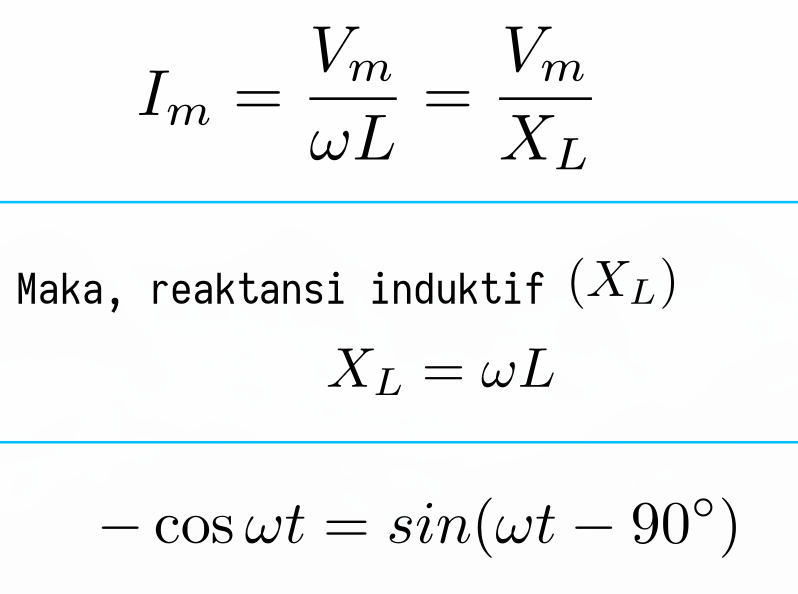
\includegraphics[width=200px]{6.png}
\end{center}

maka,
\[I=I_{\text{max}}\sin(\omega t-90\degree) \]

\begin{center}
    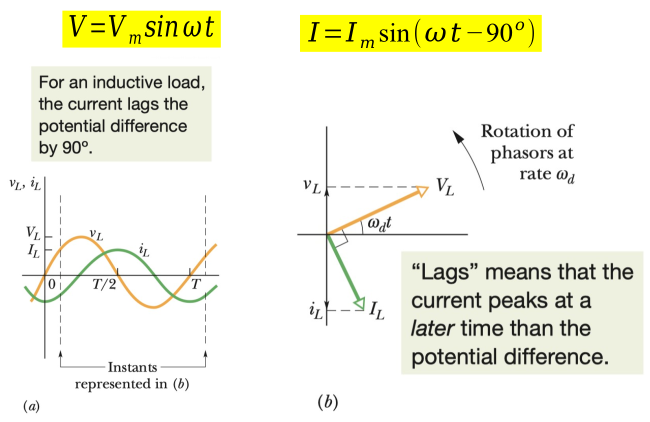
\includegraphics[width=200px]{7.png}
\end{center}

\section{Kapasitansi Dalam Rangkaian AC}%

\begin{center}
    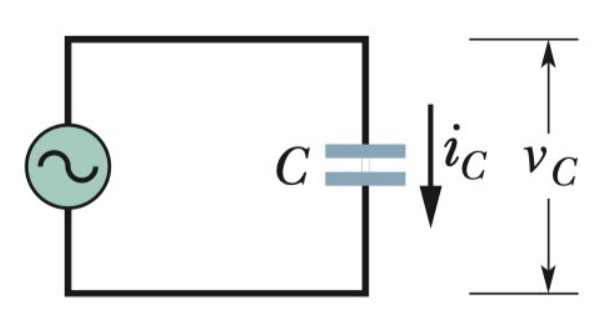
\includegraphics[width=150px]{8.png}
\end{center}

Dalam rangkaian di atas,
\[ V=V_m \sin (\omega t)\]

Dengan, $\displaystyle V=\frac{q(t)}{C}$

Sehingga,
\begin{align*}
    dV&=\frac{dq(t)}{C}\times\frac{dt}{dt}\\
    \frac{dV}{dt}&=\frac{1}{C}.\frac{dq(t)}{dt}\\
    V_m \omega\cos(\omega t)&=\frac{1}{C}.I\\
    I&= C \omega V_m \omega\cos(\omega t)\\
    I&= \frac{V_m}{X_C}C \cos(\omega t)\\
\end{align*}

Dikarenakan,
\begin{center}
    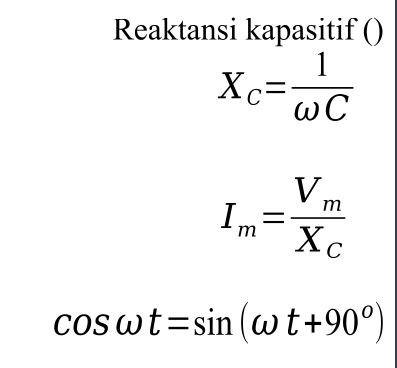
\includegraphics[width=100px]{9.png}
\end{center}

Maka,
\[ I=I_m \sin(\omega t+90\degree) \]

\begin{center}
    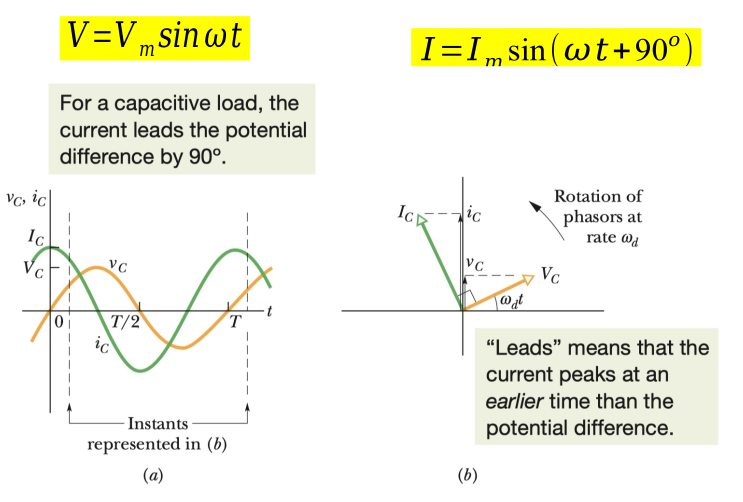
\includegraphics[width=200px]{10.png}
\end{center}

\end{document}
